% !Mode:: "TeX:UTF-8"

\chapter{绪论}

\section{课题背景与研究意义}
单人姿态估计是计算机视觉领域的热点基础问题之一,已经研究了20多年。它之所以重要,是因为有大量的应用程序可以从这种技术中受益。例如,人体姿势估计可以在人机交互和活动识别的背景下进行更高层次的推理;它也是无标记运动捕捉(MoCap)技术的基本构建块之一。MoCap技术适用于角色动画、电影和游戏,以及病理步态的临床分析等应用。

人体姿态估计具体是指基于观察图像中的人体来恢复关节和躯干。\cite{杨川2019基于深度学习的人体姿态估计技术研究}

近年来,已有大量的成果使用到了神经网络训练姿态估计,人体姿态估计在实际生活中的应用也愈发广泛。具体如下:

\begin{enumerate}
\item 虚拟试衣

\qquad \quad 随着单人姿态估计的技术越发成熟,现在一些服饰店(如优衣库、男衣邦)推出虚拟试衣服务。以便用户省去脱衣试衣的繁琐操作,另外此项技术在疫情期间网上购物的应用场景下显然有着更光明的应用前景。图~\ref{piture:1}~便是来自ICCV2021的一篇虚拟试衣论文

\begin{figure}[h]
\centering
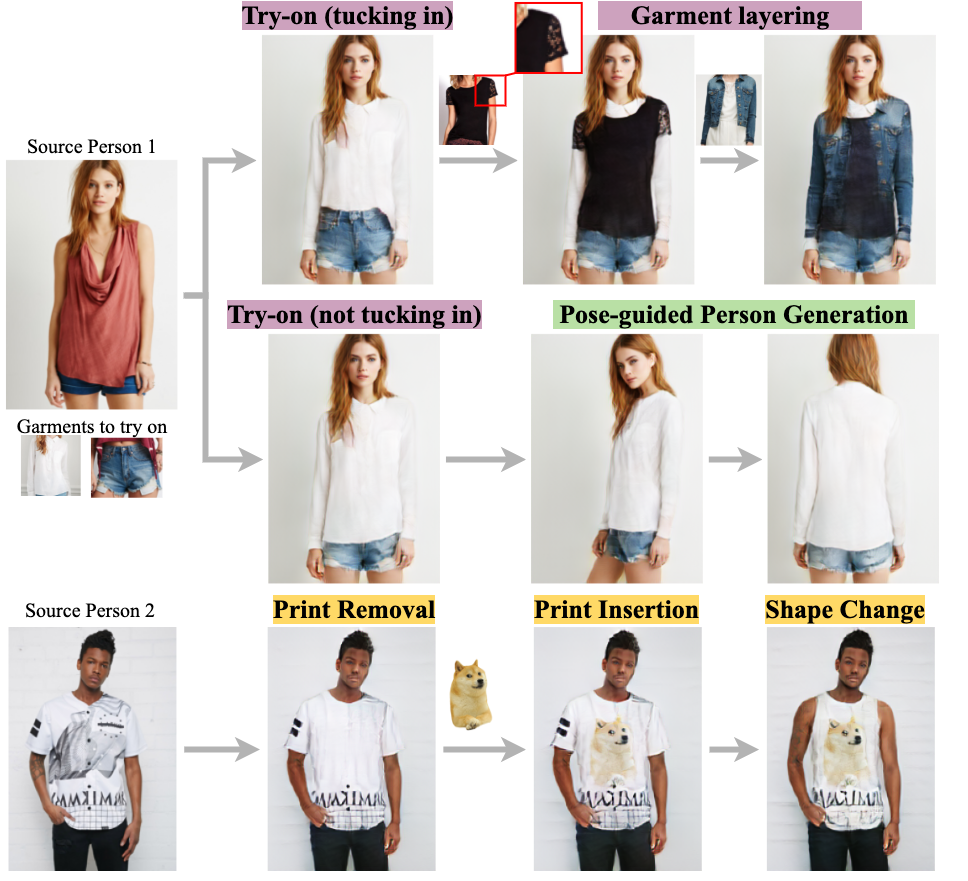
\includegraphics[width = 0.8\textwidth]{Cui_Dressing_in_Order_Recurrent_Person_Image_Generation_for_Pose_Transfer_ICCV_2021_paper_1}
\caption{不限定品类和数量的多件单品试穿,来自DiOr (Cui et al.\inlinecite{cui2021dressing})}
\label{piture:1}
\end{figure}

\item 智能安防

\qquad \quad 随着5G网络的普及,摄像头遍布公共场所,可以采集丰富的人类行为数据。现有的人体姿态估计算法已经可以分析并自动识别出监控视频中人群的活动。如存在着异常的行为,则可以即使给出异常提示或警报。\cite{戴汉彬2021基于深度学习的人体姿态估计技术研究}

\item 体育健身

\qquad \quad 疫情场景下的居家健身成为当下时代热门,如何规范、无错误动作的健身则显得尤为重要。因此,基于人体姿态估计的健身程序应运而生。该类程序运用单人姿态估计算法获取人体姿态,检测姿势是否标准,一定程度上减少了因动作不规范而引发的安全隐患。图~\ref{piture:2}~就是来自谷歌的AI健身。

\begin{figure}[h]
\centering
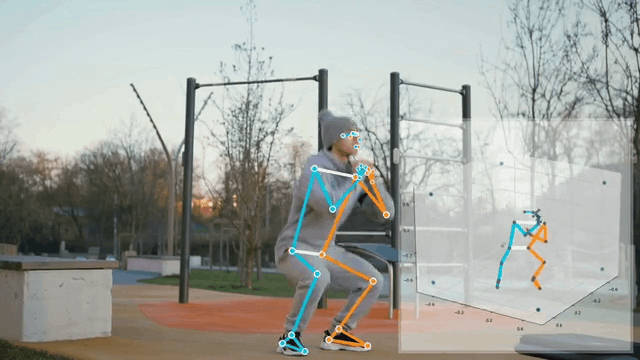
\includegraphics[width = 0.8\textwidth]{example3-13}
\caption{基于姿态估计的AI健身,来自谷歌官网}
\label{piture:2}
\end{figure}

\item VR技术

\qquad \quad 在元宇宙概念爆火的同时,也带来了一个问题,那就是VR设备动辄几万美元的费用并不是大部分人所能承担得了。作为VR体感技术的代替品,姿态估计有着得天独厚的优势,如低廉的价格、更少的硬件设备等。就目前而言,微软已有相关应用:Kinect\cite{zhang2012microsoft}。

\end{enumerate}

\section{国内外研究现状}

\subsection{基于图的人体姿态估计}

图模型、优化算法和组件外观模型是基于图的人体姿态估计方法的三个部分。该方法定义的图结构如图~\ref{piture:3}~所示。图结构模型的工作原理主要是设计一些人体部件检测器,并将各部件之间联通起来,再根据人体运动学的一些要求实现人体姿态估计。这种设计方法的主要缺点有:

\begin{enumerate}
\item 一方面,图模型结构的时间复杂度虽然较低,但是它主要提取的是HOG和SHIEFT特征,导致其无法重复使用图像的底层信息和语义信息,从而使得图像中的底层信息对于算法的制约很大。另一个,由于部件的模型较为简单,当人体运动幅度过大时,算法不能很好地识别出姿态,同一种姿态存在着多个可行解,使得图结构模型方法的应用场景比较狭隘。

\item 另一个方面,图结构模型方法基本上都是基于传统的数字图像提取特征算法,所以需要较为昂贵的专业传感设备,导致应用场景进一步受到限制。另外,这种算法通常需要多视角摄像来减少遮蔽问题,导致姿态数据的获取很是繁琐。因此,基于传统的数字图像提取特征算法来进行姿态估计无法推广,而且效率极为低效。
\end{enumerate}

\begin{figure}[h]
\centering
\includegraphics[width = 0.8\textwidth]{piture_model}
\caption{人体图结构,Felzenszwalb et al.\inlinecite{felzenszwalb2005pictorial}}
\label{piture:3}
\end{figure}

\subsection{基于深度学习的人体姿态估计}

由于技术的掣肘,在2015年之前,大部分基于深度学习的人体姿态估计都是回归精确的关键点坐标$(x,y)$,由于人体的刚性程度很低,导致这种单一方式的模型拓展性较差。因此我们主要分析15年之后的单人姿态估计算法。

MPII单人数据集是目前单人姿态估计的主流数据集之一,这可以通过计算这个数据集的PCK(Percentage of Correct Keypoints,如式(\ref{eq:1})所示)值来评估模型的优劣。目前MPII单人数据集的排名如表~\ref{performance}~所示。

\begin{equation}
\label{eq:1}
\begin{aligned}
PCK_{i}^{k}&=\frac{\sum_{p}\delta(\frac{d_{pi}}{d_{p}{def}}\leqslant T_{k})}{\sum_{p}1}\\
PCK_{mean}^{k}&=\frac{\sum_{p}\sum_{i}\delta(\frac{d_{pi}}{d_{p}{def}}\leqslant T_{k})}{\sum_{p}\sum_{i}1}
\end{aligned}
\end{equation}

\begin{table}[htbp]
\caption{Overall performance}
\label{performance}
\vspace{0.5em}\centering\wuhao
\begin{tabular}{ccccccccc}
\toprule[1.5pt]
&Head & Shoulder & Elbow & Wrist & Hip & Knee  & Ankle & Total\\
\midrule[1pt]
Pishchulin et al., ICCV'13\cite{pishchulin2013strong}& 74.3  & 49.0  & 40.8  & 34.1  & 36.5  & 34.4 & 35.2 & 44.1\\
Tompson et al., NIPS'14\cite{tompson2014joint}& 95.8  & 90.3  & 80.5  & 74.3  & 77.6  & 69.7 & 62.8 & 79.6\\
Carreira et al., CVPR'16\cite{carreira2016human}& 95.7  & 91.7  & 81.7  & 72.4  & 82.8  & 73.2 & 66.4 & 81.3\\
Tompson et al., CVPR'15\cite{tompson2015efficient}& 96.1  & 91.9  & 83.9  & 77.8  & 80.9  & 72.3 & 64.8 & 82.0\\
Hu\&Ramanan, CVPR'16\cite{hu2016bottom}& 95.0  & 91.6  & 83.0  & 76.6  & 81.9  & 74.5 & 69.5 & 82.4\\
Pishchulin et al., CVPR'16\cite{pishchulin16cvpr}& 94.1  & 90.2  & 83.4  & 77.3  & 82.6  & 75.7 & 68.6 & 82.4\\
Lifshitz et al., ECCV'16\cite{lifshitz2016human}& 97.8  & 93.3  & 85.7  & 80.4  & 85.3  & 76.6 & 70.2 & 85.0\\
Gkioxary et al., ECCV'16\cite{chain16}& 96.2  & 93.1  & 86.7  & 82.1  & 85.2  & 81.4 & 74.1 & 86.1\\
Rafi et al., BMVC'16\cite{rafi2016efficient}& 97.2  & 93.9  & 86.4  & 81.3  & 86.8  & 80.6 & 73.4 & 86.3\\
Belagiannis \& Zisserman, FG'17\cite{belagiannis2017recurrent}& 97.7  & 95.0  & 88.2  & 83.0  & 87.9  & 82.6 & 78.4 & 88.1\\
Insafutdinov et al., ECCV'16\cite{insafutdinov16ariv}& 96.8  & 95.2  & 89.3  & 84.4  & 88.4  & 83.4 & 78.0 & 88.5\\
Wei et al., CVPR'16\cite{wei2016convolutional}& 97.8  & 95.0  & 88.7  & 84.0  & 88.4  & 82.8 & 79.4 & 88.5\\
Bulat \& Tzimiropoulos, ECCV'16\cite{bulat2016human}& 97.9  & 95.1  & 89.9  & 85.3  & 89.4  & 85.7 & 81.7 & 89.7\\
Newell et al., ECCV'16\cite{newell2016stacked}& 98.2  & 96.3  & 91.2  & 87.1  & 90.1  & 87.4 & 83.6 & 90.9\\
Tang et al., ECCV'18\cite{tang2018quantized}& 97.4  & 96.4  & 92.1  & 87.7  & 90.2  & 87.7 & 84.3 & 91.2\\
Ning et al., TMM'17\cite{ning2017knowledge}& 98.1  & 96.3  & 92.2  & 87.8  & 90.6  & 87.6 & 82.7 & 91.2\\
Luvizon et al., arXiv'17\cite{DBLP:journals/corr/abs-1710-02322}& 98.1  & 96.6  & 92.0  & 87.5  & 90.6  & 88.0 & 82.7 & 91.2\\
Chu et al., CVPR'17\cite{chu2017multi}& 98.5  & 96.3  & 91.9  & 88.1  & 90.6  & 88.0 & 85.0 & 91.5\\
Chou et al., arXiv'17\cite{DBLP:journals/corr/ChouCC17}& 98.2  & 96.8  & 92.2  & 88.0  & 91.3  & 89.1 & 84.9 & 91.8\\
Chen et al., ICCV'17\cite{chen2017adversarial}& 98.1  & 96.5  & 92.5  & 88.5  & 90.2  & 89.6 & 86.0 & 91.9\\
Yang et al., ICCV'17\cite{yang2017learning}& 98.5  & 96.7  & 92.5  & 88.7  & 91.1  & 88.6 & 86.0 & 92.0\\
Ke et al., ECCV'18\cite{Ke_2018_ECCV}& 98.5  & 96.8  & 92.7  & 88.4  & 90.6  & 89.4 & 86.3 & 92.1\\
Tang et al., ECCV'18\cite{Tang_2018_ECCV}& 98.4  & 96.9  & 92.6  & 88.7  & 91.8  & 89.4 & 86.2 & 92.3\\
Zhang et al., arXiv'19\cite{zhang2019human}& 98.6  & 97.0  & 92.8  & 88.8  & 91.7  & 89.8  & 86.6  & 92.5\\
Su et al., arXiv'19\cite{su2019cascade}& 98.7  & 97.5  & 94.3  & 90.7  & 93.4  & 92.2  & 88.4  & 93.9\\
Bulat et al., FG'2020\cite{bulat2020toward}& 98.8  & 97.5  & 94.4  & 91.2  & 93.2  & 92.2  & 89.3  & 94.1\\
\bottomrule[1.5pt]
\end{tabular}
\end{table}



大体上表~\ref{performance}~中的算法可以分成两类:
\begin{itemize}
\item 基于热图的方法
\item 基于回归的方法
\end{itemize}

热力图方法能以较小的算力开销拓展到多人姿态识别,但会使得模型更复杂。

而基于回归的算法虽然计算简单,但也有一定的缺陷。最致命的是,基于回归的方法通过预测平均值并不能解决多义性问题。

Pfister et al.\inlinecite{pfister2015flowing}首次提出了回归heatmap,同时使用了网络层次较深的卷积神经网络进行姿态估计,将单人姿态估计的鲁棒性进一步提高,并且可以可视化观察训练过程,以便即使调整网络结构,避免不必要的能耗。Pfister最具创意的地方在于提出了空间融合模型,即将CNN的第三层和第七层分别提取出来再进行一次卷积操作;同时还使用了光流信息,预测出相邻帧的热力图,减少了模型的复杂度。最后经过一个池化层将对齐的热力图合成一个置信图。

Wei et al.\inlinecite{wei2016convolutional}提出了CPM(Convolutional Pose Machine)算法,使用卷积神经网络进行人体姿态估计,它的创新点在于卷积结构是高度顺序化的,表现在网络分成了多个阶段,每个阶段都会监督训练,可以更好地融合空间、纹理信息。另外还使用了多尺度处理输入,提升了模型的准确度。

Newell et al.\inlinecite{newell2016stacked}提出了SHN(Stacked Hourglass Networks)算法,使用了沙漏结构,在参数量减少的同时,又能兼顾到基于回归的姿态估计方法的准确度。SHN算法重复使用自底向上/自顶向下地网络结构,看起来像一个沙漏,故此得名。另外,同时引入了中间监督学习,从而显著提高了模型的准确率。

王晓刚组于2017年提出structured pose\cite{chu2016structured},网络结构同样是基于CNN,它在卷积层使用了几何变换核,并引入双向树概念,使得关键点的通道可以互相接受信息,从而达到信息传递的作用。与王晓刚组不同的是,Chen et al.\inlinecite{chen2017adversarial}网络结构基于GAN,性能提升效果并不显著,更多的是对于沙漏网络之后的参数微调。

Ke et al.\inlinecite{Ke_2018_ECCV}将多内容信息注意力机制迁移到卷积神经网络,得到了单人姿态估计的端到端框架,并且改进了hourglass网络架构,设计出新颖的HRUs(Hourglass Residual Units),以增加网络接受野。同时还是用了多尺度监督来训练模型,多尺度回归来优化人体结构。最后又使用了keypoint masking作为数据扩增的方式。

Tang et al.\inlinecite{Tang_2018_ECCV}设计了基于DNN的网络结构,新颖的地方在于,这个网络结构是分层组成的,并且在推理阶段使用了自下而上/自上而下。

百度研究院和香港科技大学联合于2019年出品了一篇单人pose检测文章\cite{zhang2019human}。这篇文章的贡献主要是提出了两个简单高效的模块,第一个是Cascade Prediction Fusion(CPF)网络,可以用来预测人体姿态关键点;另外一个是Pose Graph Neural Network(PGNN),用于修正预测的关键点。

2019年南京开发团队(平安科技所著)的一篇论文\cite{su2019cascade}里的算法在mpll数据集中的准确率达到93.9\%,与之前其他的单人姿态估计算法相比,准确度有着明显的提升。这主要归功于作者提出了三点创新。第一,最后将多个热图的平均值作为最后输出,提高了模型的鲁棒性;第二,联合了resnet101模型和resnet50模型,使得效果达到最佳;第三,在数据集方面,引入AI Challenger数据集起到正则化的作用。

Bulat et al.\inlinecite{bulat2020toward}设计小的block和feature map的融合方式,提人体姿态估计高计算效率和精度。该模型在MPII和LSP数据集上实现了SOTA。此外,在模型的复杂度降低三倍的情况下,运行速度提升了两倍,并且性能没有下降。在mpll数据集结果达到94.1\%。

\section{论文主要研究内容及创新点}
本文以谷歌闭源工业级模型BlazePose为切入点,优化其网络结构,完成代码复现工作,得到一个较好的模型,并利用该模型完成了对于图片、视频和摄像头实时的检测工作,并且成功将其移植到手机端、unity虚拟机器人和真实机器人上。

与之前的姿态估计算法相比,BlazePose的主要创新性工作如下:

\begin{itemize}
\item 提出了detector-tracker设计的推理通道

\qquad \quad 流程包括一个轻量级的人体姿态估计检测器和一个姿态跟踪网络。跟踪网络预测关键点坐标。当画面中第一次出现人体时,我们启动人体检测器,定位出ROI(region of interest),随后跟踪器在ROI上预测33个关键点;当画面中不是第一次出现人体(即当前帧的前一帧出现了人体),我们不会启用检测器,而是直接从上一帧的关键点推导出ROI。这样会大大提升模型的轻量化。


\item 提出了基于人脸的人检测器,

\qquad \quad 目前主流的人体姿态估计算法在检测人体的后处理步骤中,都是使用的NMS(non maximum suppression)算法,不过NMS对于非刚性物体并不是很友好,尤其是类似与人体这类关节复杂度高的姿势场景。这是因为有大量的,模糊的候选框都满足非最大值抑制的交并比阈值。

\qquad \quad 注意到人脸比较刚性,特征的对比度相对较高,所以我们假设人脸是始终可见的。对于如何检测人脸,我们使用了一个由Bazarevsky et al.提出的BlazeFace\cite{bazarevsky2019blazeface}模型。

\item 将基于热图方法和基于回归方法相结合

\qquad \quad 结合两者的优点,使用编码器-解码器网络架构来预测所有关节的热图。同时后面跟着另一个编码器,直接回归到所有关节的坐标。值得注意的是,热图分支可以在推理过程中被丢弃,使得模型足够轻量级,可以在移动端上运行。
\end{itemize}

\section{论文章节安排}

本文共五章。绪论主要介绍了论文工作的研究背景和应用场景,对国内外的人体姿态估计算法做出了一个较为详细的概况,最后概述了本项目的工作内容和创新点。

第二章介绍了有关深度学习的基础知识和基本概念以及本文用到的损失函数,激活函数,优化方法等。

第三章主要介绍了Blaze算法的推理通道,神经网络结构,人体检测器,人体拓扑结构,复现过程等。

第四章是成果展示,主要包括了五个方面:

\begin{itemize}
\item 与官方模型及其他模型的性能对比;
\item 适用于pc端的图片检测、视频检测和摄像头检测;
\item 适用于手机移动端的摄像头实时检测;
\item 在unity端虚拟机器人的检测;
\item 使用arduino开发板驱动sg90舵机完成最终的机器人姿态模仿。
\end{itemize}

% Local Variables:
% TeX-master: "../thesis"
% TeX-engine: xetex
% End: